\section{Proof-of-Work (PoW)\label{pow}}
\begin{otherlanguage}{english}
% Oikoluettu: X 
Proof-of-Work, josta tässä tutkielmassa käytetään lyhennettä PoW, on tutkielman kirjoittamisen hetkellä markkinaosuudeltaan suurin konsensusmekanismi. PoW:ta käyttää kaksi suurinta lohkoketjua: Bitcoin ja Ethereum \cite{Coingecko}.

\begin{figure}[!htbp]
\centering
\fbox{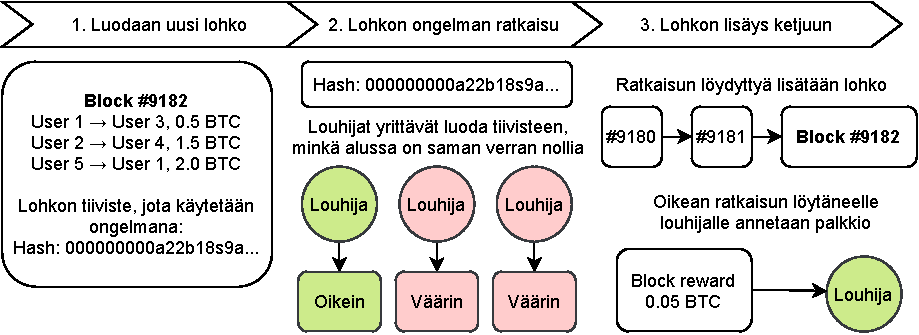
\includegraphics[width=0.98\textwidth]{proof-of-work}}
\caption{Esimerkki Proof-of-Work ja Proof-of-Space konsensusmekanismien toimintaperiaatteesta}
\label{fig_pow}
\end{figure}

\vspace{1mm}

PoW vaatii, että sen turvaamiseen osallistuvat käyttäjät, joita kutsutaan louhijoiksi (eng. \textit{miners}), ratkaisevat kryptografisen ongelman varmistaakseen, että lohkoketjuun lisätty lohko on oikea \cite{blockchain1}. Ongelman ratkaisemisen jälkeen oikean ratkaisun löytäneelle käyttäjälle annetaan palkkio (eng. \textit{block reward}). Kaavio \ref{fig_pow} näyttää millaisista vaiheista uusien lohkojen lisääminen koostuu. Tätä kokonaisuutta millä lohkoketjua turvataan kutsutaan louhinnaksi (eng. \textit{mining}) ja tämä tutkielma käyttää myös kyseistä termiä viitatessaan lohkoketjun turvaamisprosessiin. PoW-lohkoketjujen sisältämää dataa ja toimintaa esitellään tutkielman johdannossa taulukossa \ref{table-pow-database}.

Kaavio \ref{fig_pow} esittää, miten uuden lohkon luominen, varmentaminen, ja lisääminen tapahtuu. Tämä kolmeen vaiheeseen (luonti, louhinta, palkitseminen) jaettu prosessi toimii tarkemmin selitettynä seuraavalla tavalla:

\begin{enumerate}
\item Luodaan siirtotapahtumia sisältävä lohko. Taulukossa \ref{table-pow-database} esiteltiin, millaista dataa lohkoketjun lohkot sisältävät. Kaavion \ref{fig_pow} ensimmäisessä vaiheessa luodaan uusi lohko, missä louhinnan kannalta olennaisinta on siitä luotu tiiviste.
\item Louhijat pyrkivät ratkaisemaan lohkon tiivisteeseen liittyvän ongelman. Koska esimerkiksi Bitcoinissa käytetty SHA-256 tiivistealgoritmi luo annetusta merkkijonosta aina saman tiivisteen, tehdään oikean tiivisteen arvaamisesta louhijoille hankalaa lisäämällä tiivisteen alkuun jokin määrä nollia \cite{blockchain1}. Vaikeusaste määräytyy louhijoiden määrän (eli käytännössä kokonaislaskentatehokkuuden) mukaan niin, että uusi lohko varmennetaan noin kymmenessä minuutissa. Lohko varmennetaan niin, että louhijat pyrkivät luomaan tiivisteen, jonka alussa on yhtä monta nollaa kuin lohkon tiivisteessä. Koska yksi merkkijono tuottaa tiivistelagoritmilla aina saman tiivisteen, joutuvat louhijat lisäämään tiivisteeseen satunnaisen luvun, mitä kutsutaan nonceksi (eng. \textit{number once}), jolloin riittävällä määrällä yrityksiä joku louhijoista saa luotua sellaisen tiivisteen, missä on vaikeuasteen vaatima määrä nollia tiivisteen alussa. Tämä on yksinkertaistettuna esitetty kaavion \ref{fig_pow} toisessa vaiheessa.
\item Oikean ratkaisun (eli käytännössä oikean tiivisteen tuottaneen noncen) löytänyt käyttäjä lähettää vastauksensa lohkoketjulle ja vastaanottaa ratkaisun löytämisestä palkkion. Palkkioksi käyttäjä saa jonkin määrän lohkoketjun käyttämää kryptovaluuttaa itselleen. Kaavion \ref{fig_pow} viimeinen vaihe käsittelee palkkionjakoa.
\end{enumerate}

Konsensusmekanismeja vertailtaessa PoW:n eduksi mainitaan usein sen suuri hajautuneisuus. Lohkoketjuissa tyypillisesti periaatteena on, että mitä hajautuneempi lohkoketju on, sitä turvallisempi se on, sillä laajasti hajautuneisiin lohkoketjuihin on käytännössä vaikeaa kohdistaa hyökkäys \cite{51attack}. Esimerkiksi Bitcoinia vastaan hyökkääminen vaatisi, että hyökkääjä saisi käyttöönsä yli puolet Bitcoinin louhintaan käytetystä laskentatehosta. Tästä käytetään Bitcoinin tapauksessa nimitystä "51\% Attack".


Tutkielma esittelee seuraavaksi kaksi suurinta PoW-konsensusmekanismilla toimivaa lohkoketjua: Bitcoinin ja Ethereumin.

\begin{subsection}{Bitcoin\label{bitcoin}}
% Oikoluettu: X 

Bitcoin kehitettiin vuonna 2009 nimimerkillä "Satoshi Nakamoto" esiintyneen tuntemattoman tahon toimesta ja siitä julkaistiin sen toimintaperiaatetta \cite{bitcoin1, satoshibitcoin} kuvaava tutkimusartikkeli, jota kryptovaluuttakeskusteluissa kutsutaan \textit{white paperiksi}. Bitcoinin tavoitteina fiat-rahaan (perinteinen raha, kuten eurot ja dollarit) verrattuna on, että sitä voi siirtää ilman rajoituksia, sen siirtomaksut ovat alhaisia ja että jokaisella käyttäjillä on pääsy täydelliseen tilikirjaan joka sisältää kaikki tapahtumat. Näiden lisäksi valuuttaa turvaa konsensusmekanismi ja kryptografia. Kryptovaluuttana Bitcoin on myös luottamukseton (eng. \textit{trustless}), eli valuutta ei vaadi toimiakseen mitään kolmatta osapuolta johon käyttäjien täytyisi luottaa vaan se toimii hajautetusti. Tavoitteet ovat muilta osin Bitcoinissa toteutuneet, mutta siirtomaksut ovat kryptovaluutan hinnan noustua nousseet jo kymmeniin euroihin.

Bitcoinissa on vain yhdenlaisia lohkoja, eli siirtolohkoja (eng. \textit{transaction block}). Valuuttaa siirtäessään käyttäjä joutuu maksamaan siirtomaksun (eng. \textit{transaction fee}) ja siirtotapahtuma lisätään seuraavaan lohkoon, jota ei ole vielä lisätty osaksi lohkoketjua. Kun lohko lisätään osaksi lohkoketjua se varmennetaan, eli louhija ratkaisee lohkoon liittyvän pulman ja saa palkintona sen sisältämissä siirtotapahtumissa maksetut siirtomaksut sekä lohkopalkkion (eng. \textit{block reward}). Lohkopalkkioiden määrä puolittuu noin joka neljäs vuosi, ja Bitcoineja tulee olemaan kokonaisuudessaan 21 miljoonaa kappaletta \cite{satoshibitcoin}.

Bitcoinissa ongelman ratkaisemiseksi ja palkkion saamiseksi tärkein tekijä on käyttäjän louhintaan käyttämän tietokoneen laskennallinen tehokkuus \cite{bitcoin1}. Bitcoinissa palkkion saannin todennäköisyys on suoraan verrannollinen käyttäjän laskennallisen tehon suhteeseen lohkoketjun kokonaislaskentatehosta. Tästä syystä valtaosa louhijoista liittyykin niin kutsuttuihin louhintavarantoihin (eng. \textit{mining pool}). Louhintavarannoissa louhijat yhdistävät laskentatehonsa ja saavat louhintavarannon voittamista palkkioista osuutensa riippuen siitä, kuinka suuri osuus heidän laskentatehostaan on louhintavarannon kokonaislaskentatehosta.

Louhinnassa palkkion voittamisen todennäköisyyden riippuessa täysin laskennallisesta tehosta Bitcoinin louhinta on aiheuttanut kilpailua laskentatehosta käyttäjien välillä. Laitteistokilpailusta ja johtavasta asemastaan suurimpana kryptovaluuttana Bitcoin vaatiikin paljon energiaa: vuonna 2021 Bitcoinin louhinnan energiankulutuksen on arvioitu olevan 200,57 terawattituntia \cite{bitcoinenergy}, ja yksi siirtotapahtuma kuluttaa keskimäärin noin 2006,54 kilowattituntia energiaa. Mikäli Bitcoin olisi valtio, olisi Bitcoin energiankulutukseltaan suurempi kuin Thaimaa. Bitcoinin energiankulutus onkin herättänyt keskustelua lohkoketjujen ympäristöystävällisyydestä ja ollut suurena vaikuttajana siihen, miksi ympäristöystävällisempiä uusia konsensusmekanismeja on kehitetty.

Bitcoinin skaalautuvuus on myös saanut osakseen arvostelua. Bitcoin pystyy käsittelemään tällä hetkellä ainoastaan seitsemän siirtotapahtumaa sekunnissa \cite{bitcoin-tps}, ja laskettu teoreettinen maksimi Bitcoinia skaalatessa on 27 siirtotapahtumaa sekunnissa mikäli yhden lohkon koko pysyisi yhdessä megatavussa. Verrattuna siihen, että PoS-konsensusmekanismilla toimivat lohkoketjut pystyvät käsittelemään jo nyt kymmenkertaisia määriä siirtotapahtumia sekunnissa \cite{algorandtech, cardano-ouroboros} on Bitcoinin käyttämän PoW-konsensusmekanismin kohtaama kritiikki tehottomana ymmärrettävää.

\end{subsection}
\subsection{Ethereum\label{ethereum}}
\begin{otherlanguage}{english}

Ethereumin kehitti kanadalais-ukrainalainen Vitalik Buterin, ja se julkaistiin 2014 \cite{buterin2017ethereum}. Ethereum kehitettiin Bitcoinin perustalle, mutta eroaa Bitcoinista radikaalisti siinä, että Ethereum sisältää Turing-täydellisen Ethereum-virtuaalikoneen (Ethereum Virtual Machine, EVM).

Ethereum rakentuu samalle PoW-konsensusmekanille, mitä Bitcoin myös käyttää \cite{buterin2017ethereum}. Louhinta tapahtuu laskennallisesti vaativan ongelman ratkaisulla, mistä oikean ratkaisun löytänyt käyttäjä palkitaan antamalla korvauksena Ether-virtuaalivaluuttaa. Siirtotapahtumissa peritään siirron tekevältä käyttäjältä siirtomaksu, ja siirtotapahtuman lohkon ongelman ratkaissut käyttäjä palkitaan siirtomaksulla.

Ethereumin suurin ero Bitcoiniin on, että Ethereum sisältää Turing-täydellisen virtuaalikoneen \cite{buterin2017ethereum}, ja virtuaalikoneen tilaa muuttavat tapahtumat perivät myös maksuna Ether-virtuaalivaluuttaa. Virtuaalikoneelle on mahdollista rakentaa Solidity-ohjelmointikielellä applikaatioita, ja näiden applikaatioiden tilan muuttaminen perii myös maksuna Ether-virtuaalivaluuttaa. 

Koska Ethereum käyttää myös laskennallisesti vaativaa PoW-konsensusmekanismia, sen vuosittainen energiankulutus on 81.48 terawattituntia \cite{ethereumenergy}.

\end{otherlanguage}

\end{otherlanguage}